En esta secci\'on, presentaremos los resultados obtenidos en los experimentos
utilizando lo definido en la secci\'on de desarrollo.

\subsection{Nodos distinguidos}

En cada experimento se analizaron las dos fuentes de información y se definió
un criterio para distinguir un nodo de cada red. Este criterio consta en que
será distinguido el simbolo con mas probabilidad de ocurrir o equivalentemente
el simbolo que tenga menor información.

Para la fuente $S_2$ una de las hipotesis es que estos nodos "distinguidos" son
nodos especiales como routers, access points, etc. dado que estos participan
en la mayor parte de las comunicaciones con la red como con el exterior.
Por lo cual esto nos daría un método (no 100\% confiable debido a casos
atípicos) de determinar los router en una red.

Otra de las hipotesis que se presenta es que una red \textit{cableada} será
mas "compresible" que una \textit{wireless}. Para esto se mostraron el
cociente de la $\frac{H(S)}{H_{MAX}(S)}$ como se desarrollo en TODO: CITA
y se los comparo entre el mismo tipo de fuente de los distintos experimentos.

\subsection{Descripción de los Gráficos}

En cada experimentación se generaron tres tipos de resultados/graficos.

\begin{itemize}
	\item Un gráfico que muestra una representación tipo torta de la fuente, esto es, la probabilidad de ocurrencia de cada simbolo.
	\item Un gráfico tipo histograma que muestra para cada símbolo la información de este. Este grafico cuenta además con una barra
	horizontar que muestra donde se situa la Entropía de la fuente (en color naranja) y otra barra similar que muestra donde
	se situa la Entropía maxima que podria tener la fuente.
	\item Un gráfico con la topologia de los mensajes de la red. Donde los nodos son \textbf{MAC} address y las
	aristas representan un paquete de un nodo a otro
\end{itemize}

\subsection{Red hogareña}

\subsubsection{Fuente Unicast-Multicast}

 Lo siguiente corresponde a la experimentacion realizada para la fuente Unicast-Multicast en una red WiFi domestica.
 
\hspace*{-1.5cm}
 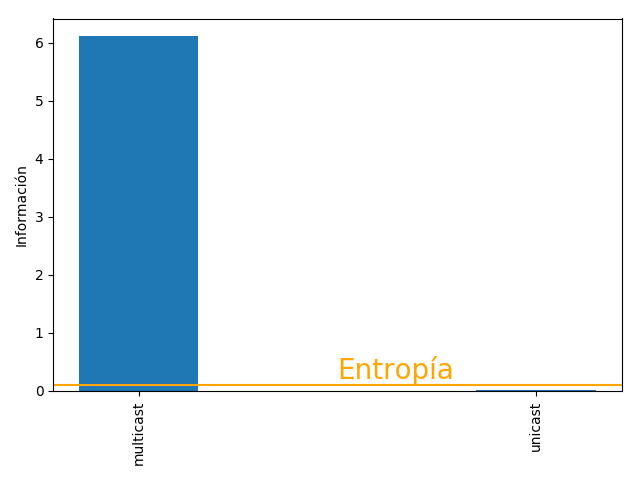
\includegraphics[scale=0.6]{../plots/mauro_s1_informacion.png}
 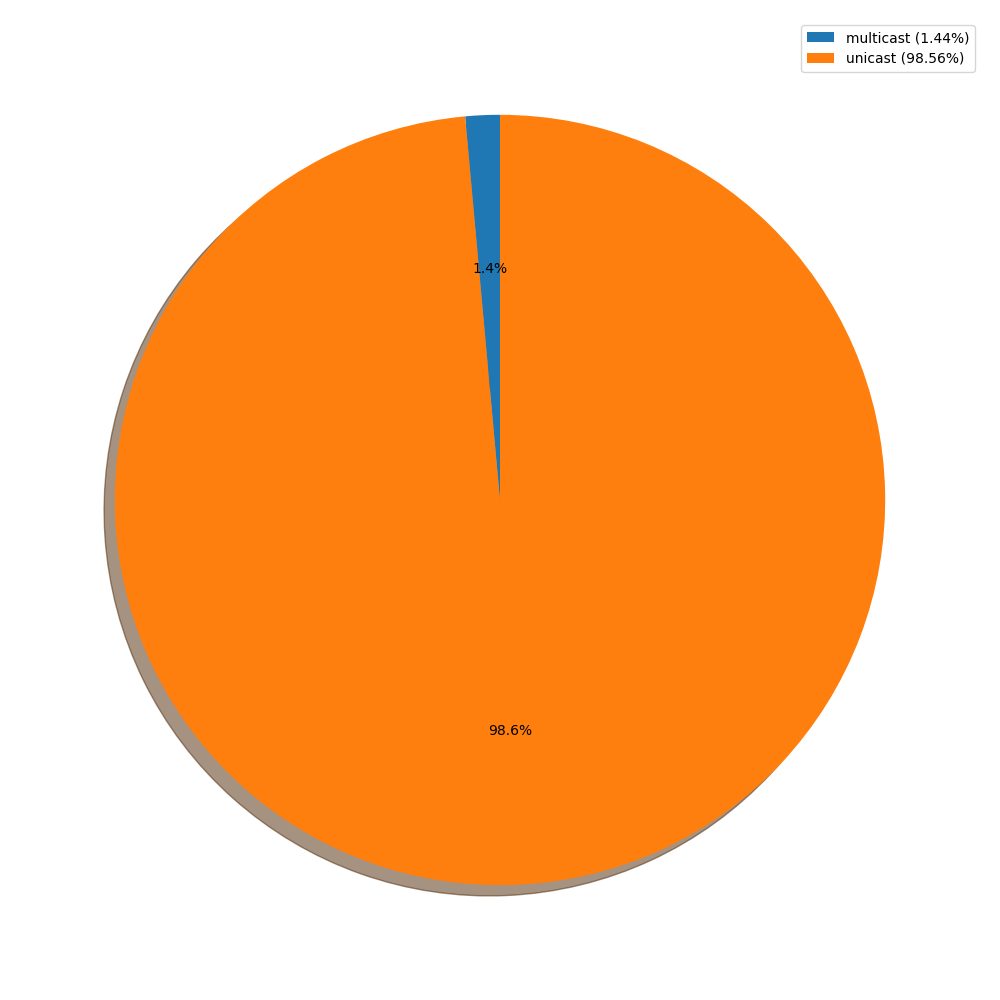
\includegraphics[scale=0.4]{../plots/mauro_s1_probabilidades.png}

 Como podemos ver los resultados obtenidos muestran una alta concentración de paquetes \textit{multicast} por sobre los \textit{unicast}. En concecuencia la entropía cae abruptamente, ya que como explicamos ésta se maximiza cuando la distribución de las probabilidades de cada símbolo es equitativa, y baja a medida que nos alejamos de ello. Nuestra primera impresion era que los paquetes \textit{unicast} iban a predominar en la captura, sin embargo esto no sucedió. Es posible que esto se deba a que la placa de red del dispositivo en el cual se tomó la muestra no hayan entrado en modo promiscuo, en consecuencia el \textit{sniffer} solo llego a capturar los paquetes cuyo destino era dicho dispositivo (y no todos los \textit{unicast} transmitidos en la red). Por el contrario los \textit{multicast} enviados por cualquier dispositivo de la red se pudieron seguir escuchando sin ningun tipo de censura.
 
\subsubsection{Fuente ARP}

\hspace*{-1.5cm}
 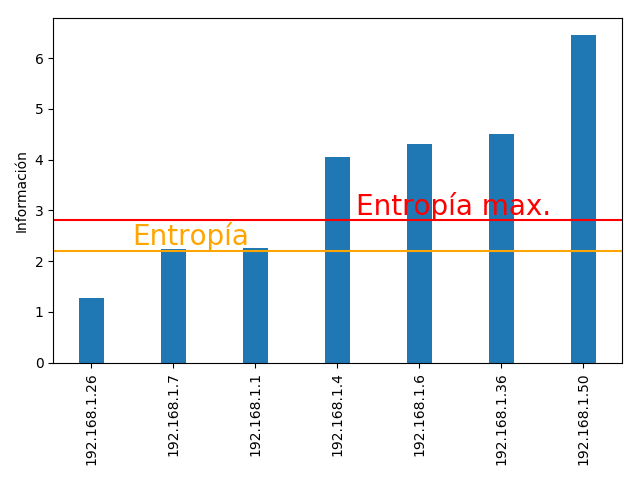
\includegraphics[scale=0.6]{../plots/mauro_s2_informacion.png}
 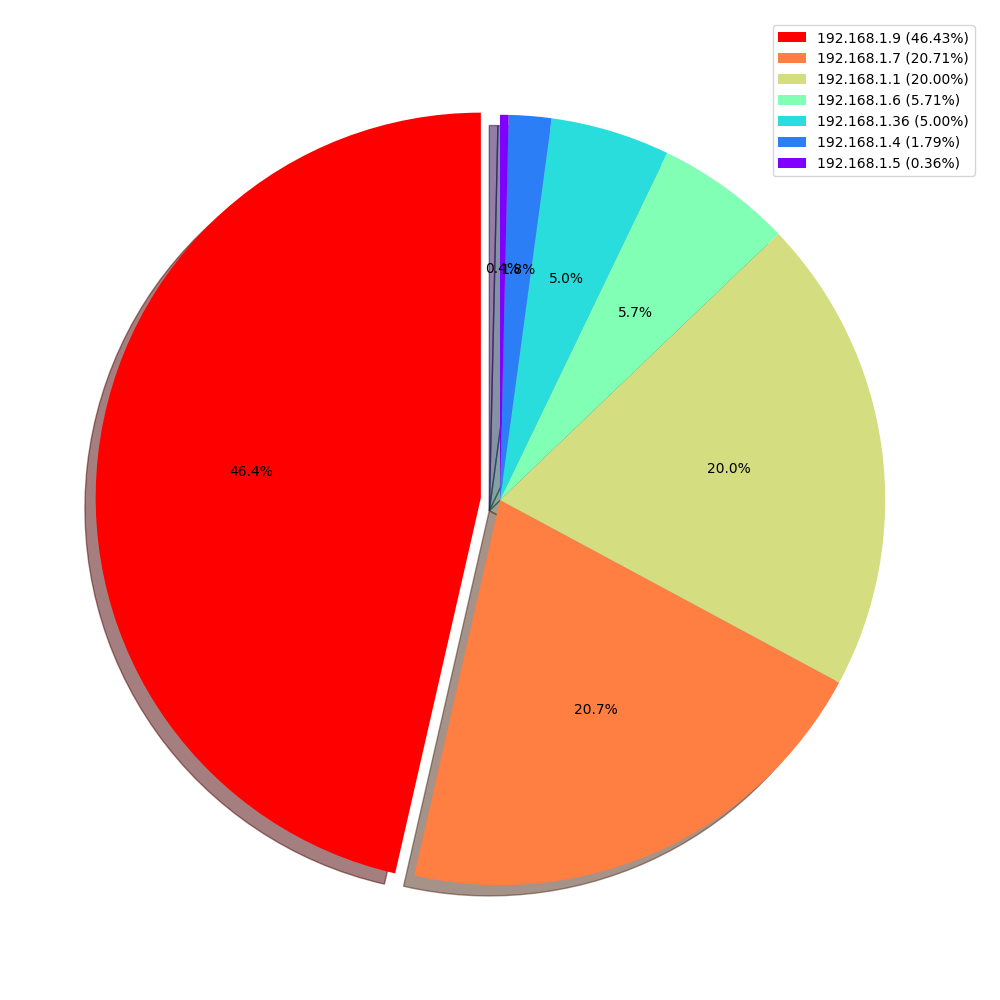
\includegraphics[scale=0.4]{../plots/mauro_s2_probabilidades.png}

\subsubsection{Topolog\'ia de la Red}
\begin{center}
 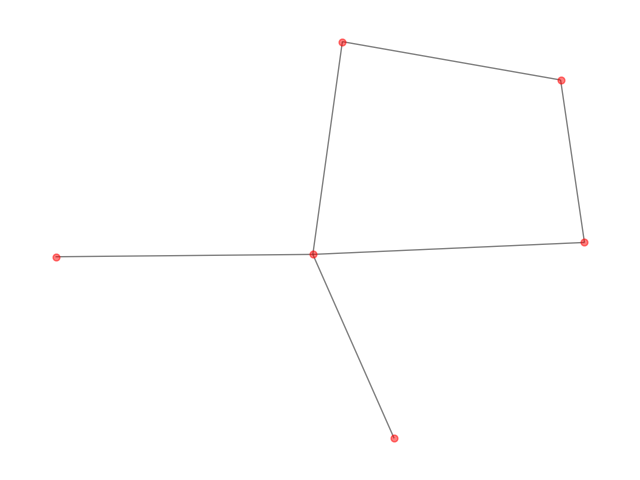
\includegraphics[scale=0.6]{../plots/mauro_s2_topologia.png}
\end{center}

\subsection{Experimento Chino}

\subsubsection{Fuente Unicast-Multicast}

\hspace*{-1.5cm}
 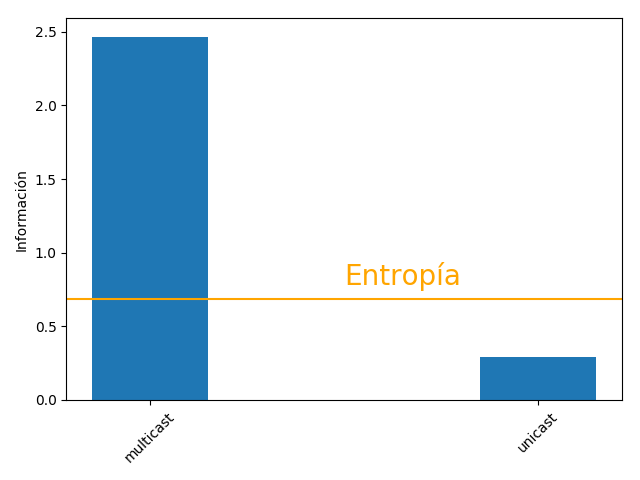
\includegraphics[scale=0.6]{../plots/trabajo_s1_informacion.png}
 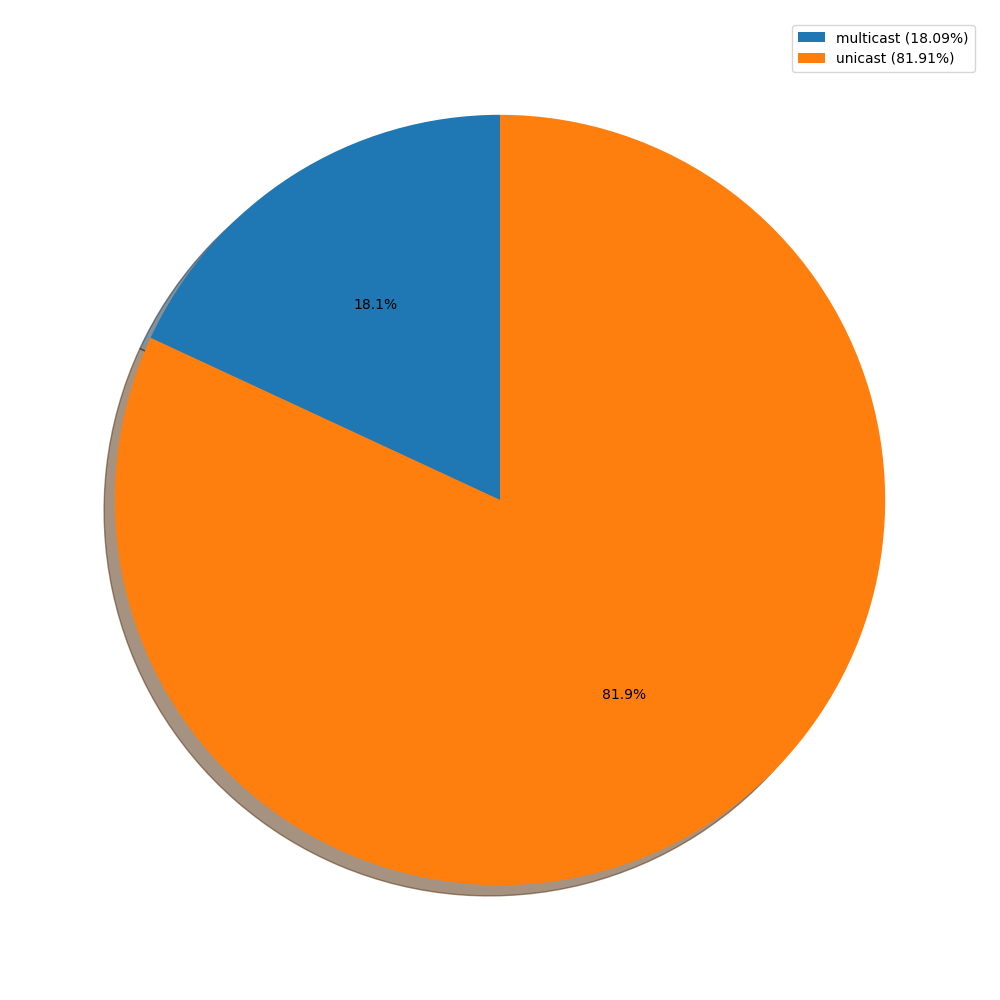
\includegraphics[scale=0.4]{../plots/trabajo_s1_probabilidades.png}

\subsubsection{Fuente ARP}

\hspace*{-1.5cm}
 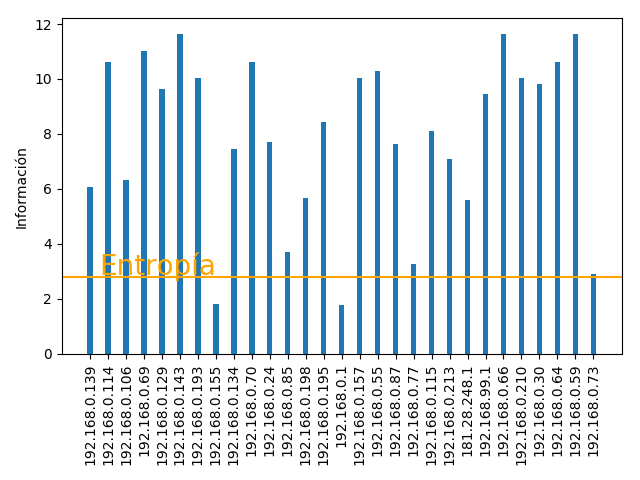
\includegraphics[scale=0.6]{../plots/trabajo_s2_informacion.png}
 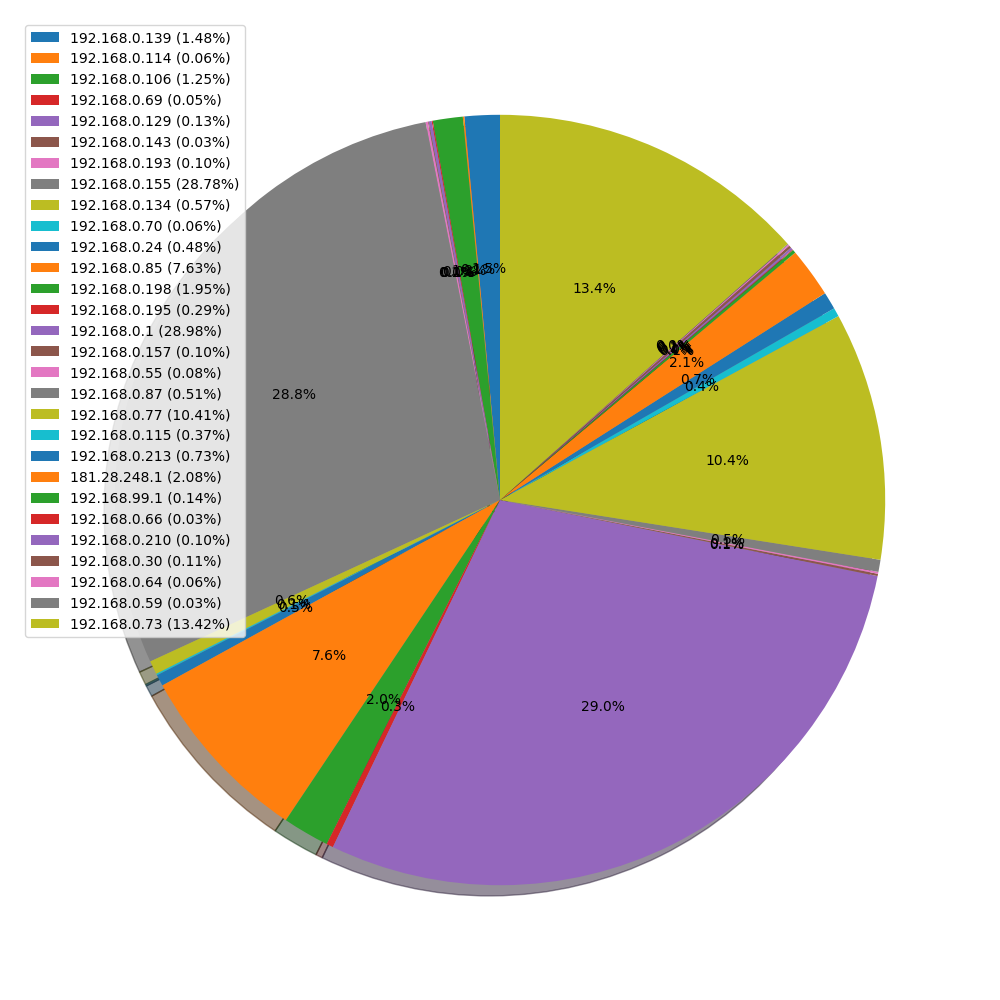
\includegraphics[scale=0.4]{../plots/trabajo_s2_probabilidades.png}


\subsubsection{Topolog\'ia de la Red}
\begin{center}
 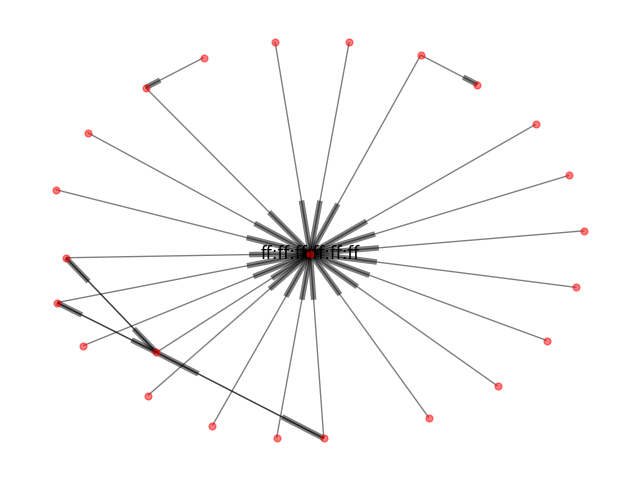
\includegraphics[scale=0.6]{../plots/trabajo_s2_topologia.png}
\end{center}

\subsection{Experimento Tavo}

Arreglar cosas